% !TEX root = ../main.tex
%\chapter{Background}
\chapter{Grundlagen}
\label{ch:basics}

Dieses Kapitel führt in die für das Framework relevanten Konzepte und Technologien ein. Zunächst wird das ArchitekturTool an sich erklärt sowie das Datenmodell des Tools. Danach wird der Begriff der \gls{eea} samt ihrer Evolution und ihres Aufbaus erläutert. Anschließend wird die Softwarearchitektur behandelt: Nach der Definition grundlegender Begriffe werden die Prinzipien der Serviceorientierten Architektur vorgestellt und darauf aufbauend die Rolle von Middleware in der Fahrzeugtechnik beleuchtet. Ein weiterer Abschnitt erläutert die Motivation, Ziele und Methoden zur Validierung von Architekturen. Den Abschluss bildet die Vorstellung des für die Implementierung verwendeten Webentwicklungs-Stacks.


\section{ArchitekturTool}
\label{sec:tool}

Das ArchitekturTool ist eine generische webbasierte Anwendung zur Modellierung, Analyse und Verwaltung von Architekturen verteilter Systeme \cite{architekturtooldocu2024}. Es ermöglicht eine vollständige Abbildung von funktionalen, softwarebezogenen und \glspl{eea}. Das Ziel ist es, eine schlanke open-source Alternative zu bieten, mit dem kleine Teams arbeiten können. Dabei soll das Tool eine weniger komplex und offen erweiterbar sein und dennoch die zentralen Funktionen kommerzieller Werkzeuge wie PREEvision (siehe Kapitel~\ref{ch:relatedWork}) zur Verfügung stellen.

Das Tool wurde im Zusammenhang mit dem AUTOTech.agil-Projekts entwickelt und legt einen besonderen Fokus auf \glspl{soa}. Es unterstützt die Modellierung und Abstimmung des Softwareentwicklungsprozesses, das Stakeholder-Management, die Pflege von Abhängigkeiten sowie die technische Qualitätssicherung.

Damit das ArchitekturTool verschiedenste Architekturen abbilden und analysieren kann, ist ein klar definiertes, strukturiertes Datenmodell notwendig. Im Folgenden wird das Datenmodell und dessen wichtigsten Elemente näher erläutert.


\subsection*{Datenmodell}

Die Grundlage zur Modellierung, Verwaltung und Analyse verteilter Architekturen im Bereich der Fahrzeugtechnik wird vom Datenmodell gebildet. Wie man in Abbildung~\ref{fig:overview_daten} erkennen kann  ist es modular und hierarchisch strukturiert, damit verschiedene Systemaspekte dargestellt werden können. Die wichtigsten Kernelemente sind dabei wie folgt:

\begin{figure}[h!]
  \centering
  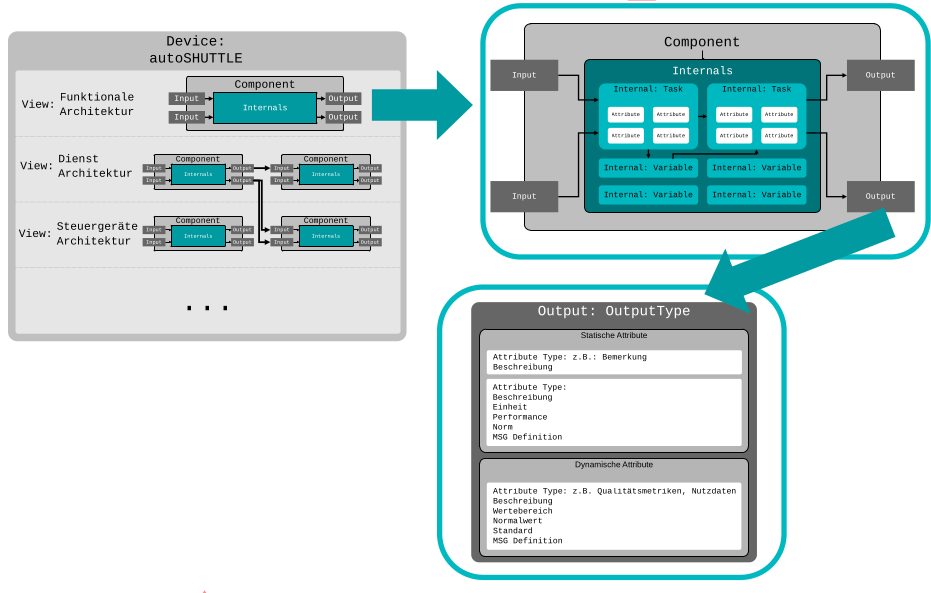
\includegraphics[width=.9\textwidth]{figures/02Grundlagen/Overview_datenmodell.png}
  \caption{Eine Übersicht des Datenmodells. (Von \cite{architekturtooldocu2024} hergenommen)}
  \label{fig:overview_daten}
\end{figure}

\begin{itemize}
  \item \textbf{Views(Sicht):} Sichten bilden das zentrale Konzept des ArchitekturTool's. Sie ermöglichen die Modellierung eines Systems aus unterschiedlichsen Perspektiven oder Abstraktionsebenen, je nachdem welche Rolle man innerhalb des Projekts hat. Sie fassen jeweils die entsprechenden Komponenten, Schnittstellen und internen Strukturen zusammen. Innerhalb des AUTOtech.agil-Projekts wurden z.B. die folgenden Sichten implementiert: funktionale-, Dienste-, Steuergerätearchitektur oder Energienetz.
  \item \textbf{Device(Gerät):} Dieses Element stellt eine Instanz eines Gesamtsystems dar, d.h. ein bestimmtes Fahrzeugmodell oder spezifisches eingebettes System. Es können mittels Devices verschiedene Formen oder physische Instanzen des gleichen Architekturmodells abgebildet werden.
  \item \textbf{Component(Komponente)} Innerhalb einer Sicht bilden Komponenten die zentralen Bauelemente. Sie repräsentieren abhängig von der gewählten Sicht beispielsweise \glspl{ecu}, Softwaredienste, Sensoren oder Aktuatoren.
  \item \textbf{Interace(Schnittstelle):} Schnittstellen beschreiben Anforderungen und Garantien, über die Komponenten miteinander kommunizieren und interagieren. Sie ermöglichen die Modellierung funktionaler, technischer oder physikalischer Beziehung, wie etwa Kommunikationskanäle, Ressourcenanforderungen oder Datenflüsse.
\end{itemize}

\section{Automobile E/E-Architektur}
\label{sect:eearchitecture}

Für alle softwaregesteuerten Funktionen innerhalb eines Fahrzeuges bildet die \gls{eea} das physikalische und logische Fundament. Sie definiert die grundlegende Organisation von Hardwarekomponenten wie \gls{ecu}, Sensoren, Energieversorgungssystemen und Kabelbäumen und steuert deren Kommunikation und Interaktion, um die erwarteten Funktionen zu realisieren \cite{jiang2019vehicle}. Diese Architektur hat im Laufe der Zeit mehrere Varianten durchlaufen und wird stetig weiterentwickelt. Im Folgenden werden die evolutionären Stufen der \gls{eea} genauer betrachtet.

\subsection*{Evolution der Architekturentwicklung}

Ursprünglich waren Fahrzeuge hauptsächlich mechanische Produkte, was sich jedoch mit der Einführung von Elektronik, wie Motorsteuergeräte und Airbags, änderte und die Ära der Elektrifizierung innerhalb der Automobilindustrie begann \cite{jiang2019vehicle}\cite{zhuRequirementsDrivenAutomotiveElectrical2021}. Zunächst waren, aufgrund der geringen Anzahl, die Verbindungen zwischen den elektronischen Komponenten meist Punkt-zu-Punkt, sprich Komponenten wurden direkt miteinander verbunden. Dies führte jedoch durch die steigende Anzahl an \glspl{ecu}, zu einem Anstieg der Komplexität und des Kabelbaums \cite{wang2024review}. Um die Kommunikationseffizienz zu verbessern und die Komplexität zu reduzieren, wurden \gls{can}-Busse eingeführt. In der Folge wurde auch an Technologien wie \gls{lin} und FlexRay entwickelt und eingesetzt, um die verschiedenen Kommunikationsanforderungen zu erfüllen, sodass Komponenten innerhalb einer Domäne Informationen gemeinsam nutzen \cite{wang2024review}\cite{zhuRequirementsDrivenAutomotiveElectrical2021}.

\begin{figure}[h!]
  \centering
  \begin{subfigure}{.5\textwidth}
    \centering
    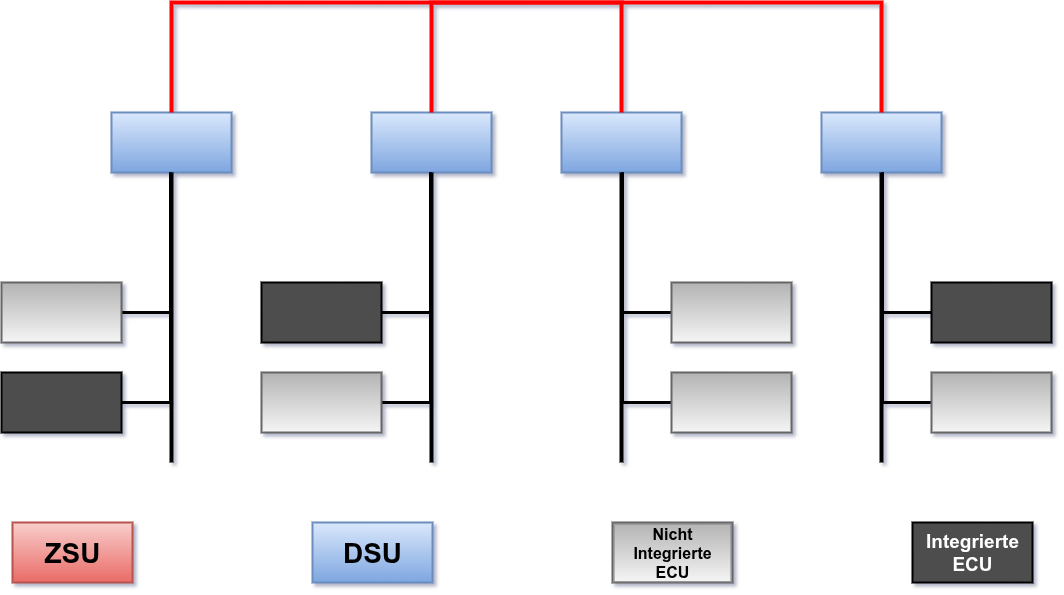
\includegraphics[width=\linewidth]{figures/02Grundlagen/Domainbasiert.drawio.png}
    \caption{Domänenbasierte \gls{eea}}
    \label{fig:deea}
  \end{subfigure}%
  \begin{subfigure}{.5\textwidth}
    \centering
    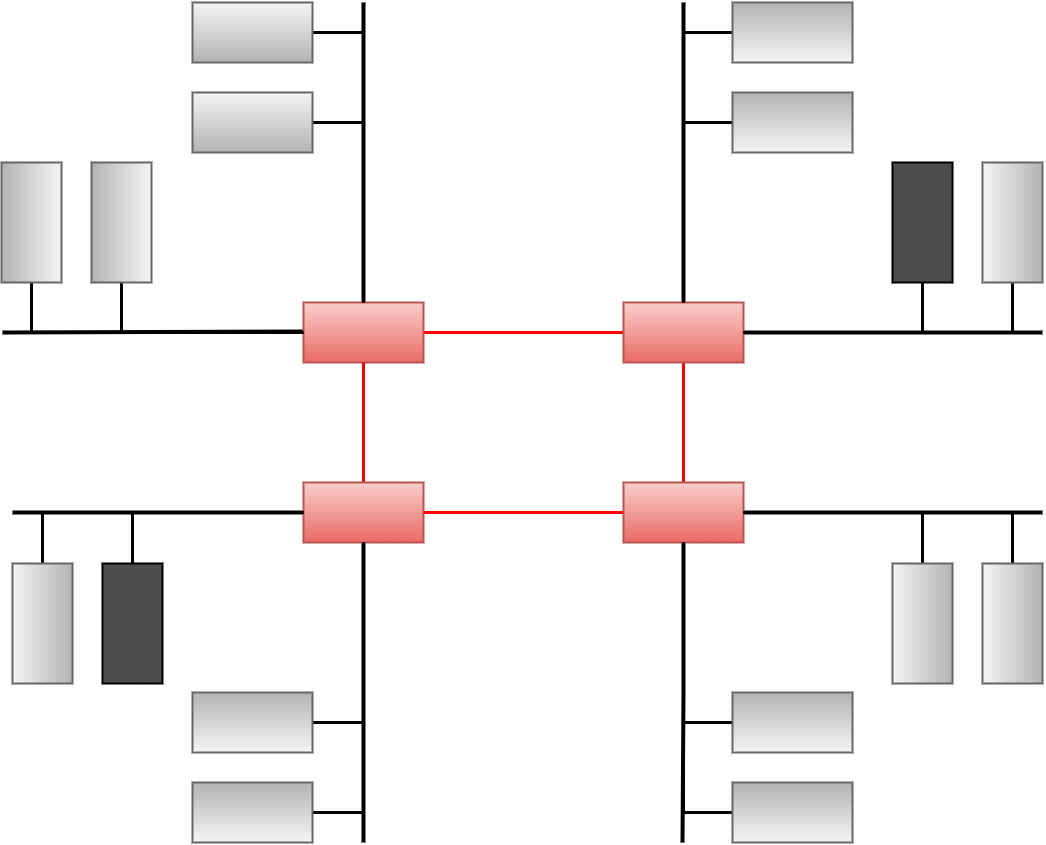
\includegraphics[width=.75\linewidth]{figures/02Grundlagen/Zonenbasiert.drawio.png}
    \caption{Zonenbasierte \gls{eea}}
    \label{fig:zeea}
  \end{subfigure}
  \caption{Vergleich zwischen funktionsorientierter (Domäne) und positionsorientierter (Zone) E/E-Architektur(Nachgezeichnet von \cite{wang2024review})}
  \label{fig:eea}
\end{figure}


Das Konzept der Funktionsdomäne rückte, aufgrund der wachsenden Komplexität und Funktionen immer stärker in den Vordergrund. Wie Abbildung~\ref{fig:deea} veranschaulicht, \glspl{ecu} und Funktionen wurden in Domänen wie Fahrwerk, Karosserie und Infotainment unterteilt \cite{jiang2019vehicle}. Durch die Nachfrage nach domänenübergreifender Kommunikation wurde die Gateway-Funktion, welche zuvor von einzelnen \glspl{ecu} übernommen wurde, zunehmend in einem dedizierten, zentralen Gateway gebündelt \cite{jiang2019vehicle}\cite{zhuRequirementsDrivenAutomotiveElectrical2021}.
Obwohl dieser Ansatz die Mainstream-Lösung war, führte die Zunahme der Funktionen und Rechenanforderungen zu einer starken Zunahme der \glspl{ecu}. Dies führte zu komplexen Kabelbäumen mit erhöhtem Gewicht und Kosten. Zudem konnte der Ausfall des zentralen Gateways einen Zusammenbruch des gesamten Netzwerks verursachen.

Um diesem Problem entgegenzuwirken, wurden \glspl{dcu} eingeführt, welche Funktionen einiger \glspl{ecu} innerhalb einer jeweiligen Funktionsdomäne integrieren und somit die Anzahl der \glspl{ecu} und die Belastung der Gateways reduzieren \cite{bandur2021making}\cite{jiang2019vehicle}\cite{wang2024review}. Um die bestmögliche Kommunikation zu garantieren, werden \glspl{dcu} über das Automotive Ethernet mit dem zentralen Gateway verbunden, welches eine höhere Bandbreite bietet.

Ein weiterer Ansatz, der neben der domänenbasierten Architektur existiert, ist die zonenbasierte Architektur. Um Komplexität und das Gewicht der Verkabelung zu reduzieren, werden Komponenten anstatt nach Funktionen, basierend auf ihrer physischen Position innerhalb des Fahrzeuges unterteilt \cite{wang2024review}\cite{jiang2019vehicle}. Abbildung~\ref{fig:zeea} zeigt diesen Ansatz, bei dem \glspl{zsu} die Funktionen übernehmen, die in den entsprechenden physischen Zonen stattfinden. Auch hier wird die Kommunikation über das Automotive Ethernet durchgeführt. Dieser Ansatz reduziert die Anzahl der \glspl{ecu} und Kabelaufwand (Anzahl, Länge, Gewicht) und verringert so die Komplexität der \gls{eea} deutlich.

Erst die Evolution der \gls{eea} ermöglicht moderne Softwarekonzepte. Das folgende Unterkapitel beschreibt daher die Softwarearchitekturen, die diese neue Hardware-Basis nutzt.

\section{Softwarearchitekturen in Fahrzeugen}
\label{sect:sa}
Die allgemeine Definition einer Softwarearchitektur ist nach Bass et al. \cite{bass2021} eine systematische Gliederung eines Softwaresystems in einzelne Bausteine, die Festlegung ihrer Schnittstelle sowie die Prinzipien, nach denen diese Komponenten zusammenwirken und organisiert sind. Seitdem sich der Schwerpunkt von Fahrzeugen weg von mechanikzentrierten Systemen bewegt hat und hin zu intelligenten, softwaredefinierten Plattformen, gibt es innerhalb der Automobilindustrie einen großen Fortschritt bezüglich der Softwarefunktionalität \cite{rumezOverviewAutomotiveServiceOriented2020}\cite{broy2006}. Um bei diesem Fortschritt den Überblick zu behalten, ist eine fundierte Softwarearchitektur unerlässlich.

Zu Beginn setzte man auf klassische, geschichtete Architekturen wie AUTOSAR Classic, jedoch merkte man mit dem Aufkommen des Konzepts eines \gls{sdv} sowie der steigenden Software-Komplexität, dass die klassische Softwarearchitektur an ihre Grenzen stieß  \cite{rumezOverviewAutomotiveServiceOriented2020}. Es gibt einige Gründe, wie die starre, monolithische Schichtenstruktur: Funktionen sind fest an Schichten gebunden, was Anpassungen einzelner Komponenten oder den Austausch von Modulen kaum umsetzbar machte.

In diesem Unterkapitel wird ein Einblick in die \glspl{soa} gegeben, die beschriebenen Schwächen der klassischen Softwarearchitektur überwinden. Anschließend wird die Middleware erläutert, die als technische Vermittlungsschicht dient.

\subsection{Serviceorientierte Architektur}
\label{subsect:soa}
Die Notwendigkeit, Softwaremodule dynamisch bereitzustellen erfordert einen flexiblen Ansatz. Hier setzt die \gls{soa}, welche bereits in der Webentwicklung fester Bestandteil ist, an. Nach Rumez et al.\cite{rumezOverviewAutomotiveServiceOriented2020} handelt es sich um ein Architekturmuster, bei dem Anwendung als lose gekoppelte, wiederverwendbare Dienste organisiert werden. Jeder Dienst bietet eine klar definierte Funktionalität über gut beschriebene Schnittstellen und kann zur Laufzeit von beliebigen Clients genutzt werden.

Im Gegensatz zum klassischen signalorientierten Ansatz, bei dem die Konfiguration der Kommunikationspfade vollständig statisch zur Design-Zeit erfolgt, setzt der \gls{soa}-Ansatz auf eine dynamische Konfiguration während der Laufzeit \cite{rumezOverviewAutomotiveServiceOriented2020}. Durch das dynamische Aufrufen von Diensten zur Laufzeit erhält die Architektur mehr Flexibilität. So lassen sich Funktionen einfacher hinzufügen, entfernen oder bearbeiten, ohne dass eine komplette Neuzuweisung der Software erforderlich ist. Dank der Middleware-Schicht, auf die im nächsten Abschnitt näher eingegangen wird, sind die verschiedenen Anwendungen unabhängig von dem Steuergerät, auf dem ein Dienst läuft, sowie vom zugrunde liegenden Netzwerk aufgebaut \cite{kugeleModelbasedResourceAnalysis2021}. Diese Entkoppelung von der Plattform ermöglicht es der Software, wiederverwendbar und portierbar zu sein \cite{cebotari2020}. Ein weiteres Merkmal des \gls{soa}-Ansatzes sind Kommunikationsmuster, die Daten nur bei Bedarf übertragen \cite{rumezOverviewAutomotiveServiceOriented2020}. Im Gegensatz dazu verschickt die klassische Softwarearchitektur in zyklischen Abständen Daten, selbst wenn kein Empfänger vorhanden ist. Dadurch wird die entstehende Netzwerklast auf das Nötigste reduziert werden, was die Effizienz  steigert. Darüber hinaus kapselt jeder Dienst hinter einer Schnittstelle eine klar definierte Funktionalität. So lassen sich diese Dienste in unterschiedliche Kontexte und Projekten wiederverwenden, wodurch der Entwicklungs- und Testaufwand gesenkt wird \cite{rumezOverviewAutomotiveServiceOriented2020}\cite{cebotari2020}. Ein weiterer Vorteil ist die Integration externer und On-Demand-Dienste: \gls{soa} unterstützen die dynamische Anbindung von Backend- und Cloud-Diensten, welche weitgehend transparent ist \cite{rumezOverviewAutomotiveServiceOriented2020}\cite{henle2022}. Außerdem lassen sich \gls{soa} an wachsenden Anforderungen anpassen ohne dass das Gesamte System neu zu strukturieren. Aus den genannten Gründen erweißt sich die \gls{soa} als flexiblere und anpassungsfähiger als die klassische Variante der Softwarearchitektur.

Um die Vorteile der \gls{soa} realisieren zu können benötigt es eine Zwischenschicht zwischen Anwendung und Netz. Im folgenden Abschnitt wird die Middleware-Schicht untersucht, welche die \gls{soa}-Prinzipien technisch umsetzt. Dabei wird zunächst auf Aden ufbau und die Funktionen eingegangen.

\subsection{Automobile Middleware}
\label{subsect:middle}
Innerhalb moderner, verteilter Softwaresysteme ist die Middleware-Schicht eine wichtige Vermittlungsebene. Neely et al. \cite{neely2006adaptive} definieren die Middleware als Schicht zwischen Anwendungssoftware und Systemsoftware. In Systemen mit Netzwerkanbindung vermittelt sie zusätzlich zwischen Anwendungssoftware, Betriebssystem und Netzwerkkommunikationsschichten. Dabei liegt ihre Hauptaufgabe darin, die Komplexität des zugrunde liegenden Systems zu abstrahieren. Im Bereich der Fahrzeugtechnik wird die Middleware noch einmal in zwei Sub-Schichten unterteilt \cite{kluner2024moderna}:
\begin{itemize}
  \item Kommunikations-Middlewares (untere Schicht), die den Datenaustausch zwischen \glspl{ecu} organisieren und \gls{qos}-Funktionen bereitstellen.
  \item Architekturplattformen (obere Schicht), die umfassende Frameworks für die Entwicklung und Bereitstellung automobiler Softwaresysteme liefern.
\end{itemize}
Nun wird untersucht, wie die Kommunikations-Middlewares und Architekturplattformen konkret arbeiten.

\begin{figure}[h!]
  \centering
  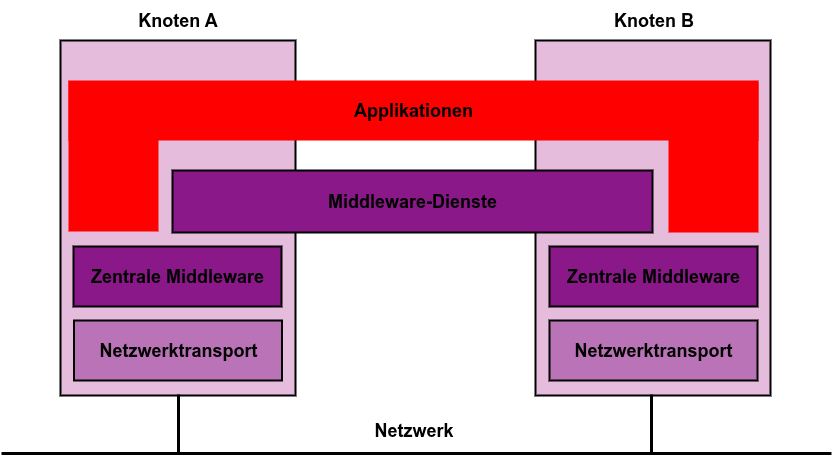
\includegraphics[width=\textwidth]{figures/02Grundlagen/Middleware_Scheme.drawio.png}
  \caption{Schematische Darstellung einer serviceorientierten Middleware-Architektur (Nachzeichnung von \cite{neely2006adaptive})}
  \label{fig:middleware}
\end{figure}

Als untere Sub-Schicht sorgt die Kommunikations-Middleware die in Abbildung~\ref{fig:middleware} aus der Zentrale-Middleware und Netzwerktransport besteht, dafür, dass sämtliche Details des Datenaustauschs im \gls{ivn} abstrahiert und Anwendungen von der zugrunde liegenden Netzwerktopologie entkoppelt sind. Sie sorgt zudem dafür, dass strukturierte Daten wie z.B. Sensormesswerte automatisch seralisiert und über Ethernet, CAN-Gateway oder Shared-Memory-Kanäle verteilt werden. Außerdem ermöglicht sie die Definition und Einhaltung von \gls{qos}-Parametern. Des Weiteren sorgt ein intelligentes Routing- und Topologie-Management auf der Netzwerk-Ebene dafür, dass Nachrichten den bestmöglichen Pfad für die Übertragung wählen, während ein Real-Time-Scheduler die Übertragungen koordiniert.

Mit der Kommunikations-Middleware als Basis, löst die Architekturplattform Herausforderungen in Bezug auf die Entwicklung von Automobil-Softwaresystemen. Sie stellt eine umfassende Laufzeitumgebung bereit und bietet Entwicklern standardisierte Dienste und APIs. Das Ziel ist es die bestehende Komplexität weiter zu verringern, sodass Entwickler den Fokus auf die Anwendungslogik setzen können, anstatt sich mit systemnahen Aufgaben zu beschäftigen. Abgesehen von der Kommunikation, gehört zunächst das umsetzen der Software-Designmustern, wie das zuvor angesprochene \gls{soa}-Prinzip, zu den Kernaufgaben. Ebenso Ressourcenmanagement und Orchestrierung , bei der die Ressourcen von inaktiven Diensten freigegeben werden. Das Ziel hierbei ist eine situationsabhängige optimale Ressourcenzuweisung. Als nächstes ist die deterministische Ausführung sowie die Unterstützung bei der Einhaltung von Echtzeitanforderung zu nennen, um Verzögerungen im Softwaresystem zu vermeiden. Des Weiteren bietet sie oft Funktionen zur Cybersicherheit, wie Authentifizierung, Zugriffskontrolle, Verschlüsserung etc. an um Schwachstellen innerhalb des \glspl{ivn} zu reduzieren. Darüber hinaus sorgt die obere Schicht dafür, dass Over-the-Air-Updates, Installation/Deinstallation von Software-Paketen, sowie die Konfiguration von Anwendungen während der Laufzeit durchgeführt werden und bietet dementsprechend Funktionen an. Eine weitere wichtige Aufgabe ist die Verwaltung des Systemzustands und die Überwachung des Lebenszyklus von Softwarekomponenten. Nicht zuletzt bietet die Architekturplattform Entwicklungstools an, welche für die Entwicklung und Bereitstellung verwendet werden.

\section{Validierung von Architekturen}
\label{sect:validerung}

Wie bereits zu Beginn der Arbeit dargelegt, ist die frühzeitige Prüfung von Architekturen von entscheidender Bedeutung. Das technische Ziel der Architekturvalidierung ist daher, die Korrektheit und Konsistenz eines Systementwurfs anhand definierter Qualitätsmethoden, wie  ISO 26262 für funktionale Sicherheit oder ISO 25010 was sind die Zielefür Softwarequalität, zu bewerten, noch bevor die Implementierung beginnt \cite{venkitachalam2015}. Dieses Ziel lässt sich in die folgenden Teilziele unterteilen: Früherkennung von Fehlern, Kostenreduzierung, Sicherstellung von Qualität und Standardkonformität, Verifikation des Systemverhaltens und der Anforderungen, Beherrschung der Systemkomplexität und Verbesserung des Verständnisses\cite{venkitachalam2015} \cite{Kan19} \cite{bucher2019crosslayera}.

Zur Gewährleistung der Gültigkeit von automobilen Systemen existieren verschiedene Validierungsansätze. Dazu zählen unter anderem die Struktur- und Konsistenzprüfung,  die Quantitative Analyse und Metrik, Sicherheits- und Zuverlässigkeitsanalysen, die verhaltensbasierte Validierung sowie die Versionsvalidierung. Im Rahmen dieser Arbeit wird der Fokus auf die Anforderungs- und Design-Validierung gelegt.

\subsection*{Anforderungs- und Design-Validierung}

Diese Validierung befasst sich mit der Überprüfung von Anforderungen und der Qualität von Architektur-Entwürfen \cite{ahrens2013objective}\cite{knieke2022managed}. Sie stellt sicher, dass funktionale und nicht-funktionale Anforderungen, wie Skalierbarkeit, Erweiterbarkeit und Portabilität, in der Softwarearchitektur berücksichtigt werden. Dabei beginnt der Vorgang oft mit der Spezifikation von Anforderungen, anschließend erfolgt die Architekturmodellierung. Ein zentrales Verfahren hierbei ist die Traceability Analyse, welche überprüft, ob alle Anforderungen im Architekturmodell abgebildet sind und jedes Element in der Architektur auf mindestens eine Anforderung zurückgeführt werden kann \cite{vogel2021metrics}.

\section{Webentwicklungs-Stack}

UmUm die Integration des erweiterbaren Validierungs-Frameworks in das bestehende System zu ermöglichen, wird im Folgenden der eingesetzte Technologie-Stack des webbasierten Architekturtools vorgestellt. Die Anwendung basiert vollständig auf JavaScript bzw. TypeScript und folgt einer klassischen Drei-Schichten-Architektur bestehend aus Frontend, Backend und Datenbank.

\subsection*{Frontend}

Zur Entwicklung der \gls{gui} des ArchitekturTools wird das JavaScript-Framework \textit{ReactJS}\footnote{https://react.dev/learn} genutzt. React ist ein populäres Frontend-Framework, dessen zentrales Konzept die komponentenbasierte Architektur ist. Dabei wird die \gls{gui} in kleine, wiederverwendbare und in sich geschlossene Bausteine, auch Components genannt, zerteilt. Für die visuelle Darstellung dieser Komponenten wird \textit{CSS}\footnote{https://www.w3.org/Style/CSS/} verwendet, eine Stylesheet-Sprache, die das Design vom strukturellen Aufbau trennt und dabei Farben, Schriftarten und das Layout der \gls{gui} definiert. Dabei nutzt React zur Aktualisierung der Ansicht ein virtuelles Document Object Model, wodurch bei Änderungen nur die betroffenen Bauteile der Webseite neu geladen werden.

\subsection*{Backend}

Die Backend-Logik des Tools wird die JavaScript-Laufzeitumbgebung \textit{Node.js}\footnote{https://nodejs.org/en} verwendet. Node.js ermöglicht die serverseitige Ausführung von JavaScript und bildet damit das Fundament für die ereignisgesteuerte, asynchrone Verarbeitung von Anfragen. Darauf aufbauend wird das Webframework \textit{Express.js}\footnote{https://expressjs.com/} genutzt, welches eine strukturierte Definition von Routen und Middlewares ermöglicht. Es dient als Hauptkomponente zur Bereitstellung der \gls{api}-Endpunkte, über die das Frontend mit dem Backend kommuniziert. Für einen einfacheren Zugriff auf die Datenbank wird das objekt-relationale Mapping-Tool \textit{Prisma ORM}\footnote{https://www.prisma.io/} verwendet. Prisma übersetzt JavaScript-Anfragen in SQL-Befehle und ermöglicht somit eine typensichere und leistungsfähige Interkation mit der relationalen Datenbank.


\subsection*{Datenbank}

\textit{PostgreSQL}\footnote{https://www.postgresql.org/} wird bei dem Tool als Datenbank genutzt, da es sich um ein objektrelationales Open-Source-Datenbanksystem handelt, das sich durch hohe Stabilität und umfangreiche Erweiterbarkeit auszeichnet. PostgreSQL dient als Speicherkomponente des ArchitekturTools und verwaltet alle strukturierten Daten, wie Informationen zu Fahrzeugkomponenten, Verbindungen oder Sichten. Die relationale Struktur ermöglicht die Realisierung von komplexen Anfragen und Verknüpfungen. In Verbindung mit Prisma wird ein typensicherer Zugriff auf die Datenbank gewährleistet.